\section{Results}
\label{sec:results}

\subsection{The size of the 21 tests}
\label{sec:rs-size}

\Cref{tab:main-results} gives the size of each test at the boundary of its null, and \cref{fig:size-forest} draws it against the level and the bound.
Three counts answer how many of the \nTests{} tests hold their size, and they differ because the evidence differs, not because the tests do.
On the committed cells of \nNullReps{} repetitions, the screen of \cref{alg:judgement} passes \nHoldCellRule{} tests and the definition of \cref{def:holds} shows \nHoldCellDef{} holding.
On the pool of the replication of \cref{sec:rs-seeds}, \nRepsPooled{} repetitions per test, the screen passes \nHoldPoolRule{} and the definition shows \nHold{} holding.
The paper reports the last: on the best evidence it has, \nHold{} of the \nTests{} tests hold their size and \nNotHold{} do not.
The counts fall as the evidence grows for two reasons.
The first is the number of repetitions: the definition sees an excess of \detIntFiveFour{} points at 5\,\% in a cell of \nNullReps{} repetitions and of \detIntFiveTwoHundredK{} points in the pool, so the pool shows excesses that a cell cannot.
The second is the tolerance of the screen, which at any number of repetitions accepts a larger excess than the definition does: at \nRepsPooled{} repetitions and the 5\,\% level it passes a rate of up to \boundFivePool\,\%, while the definition shows an excess from a rate of \intRateFiveTwoHundredK\,\%.
That is why \nPoolDefOnly{} tests, DeLong's test (\pooledDel\,\% at 5\,\%) and the characteristic stability index (\pooledCsiOne\,\% at 1\,\%), are shown above their level by the definition and pass the screen.
The tolerance has a reason, the false flag probability of \cref{prop:false-flag}, and a price: the definition expects at most \expFalseAbove{} of the 21 tests to be shown above their level by chance if every test had exactly its level, so DeLong's test and the characteristic stability index, whose lower interval limits clear the level by the least (\pooledDelLo\,\% against 5\,\% and \pooledCsiLoOne\,\% against 1\,\%), are the least certain of the nine, and the seven that the screen also flags are not explained by chance.
The nine tests that do not hold their size on the pool are the Jeffreys test, the normal test over five years, the chi-square test over grades, Hosmer--Lemeshow, Spiegelhalter, the population stability index, the Markov-order test, DeLong's test and the characteristic stability index (\cref{tab:seed-replication}).
Two of them exceed their level by more than a fraction of a point.
The Jeffreys test of the default probability has a simulated rate at 1\,\% of \jeffSimOne\,\% in the committed cell, inside the bound of \boundOne\,\%, but its exact size at 1\,\% for 1,000 obligors at a probability of default of 1\,\% is \jeffExactOne\,\%: the posterior probability of the Jeffreys prior is a Bayesian quantity, and as a frequentist test of a discrete count its size moves with the number of obligors.
A cell of \nNullReps{} repetitions shows a true size of \jeffExactOne\,\% at 1\,\% with probability only \jeffDetect\,\% by the screen and \jeffDetectInt\,\% by the definition, and the exact value, placed beside the rate, is what decides.
The normal test over five years rejects \normFive\,\% of the correct models at 5\,\% in the committed cell (Wilson interval \normLoFive\,\% to \normHiFive\,\%) and \normOne\,\% at 1\,\%, against bounds of \boundFive\,\% and \boundOne\,\%, and \pooledNorm\,\% at 5\,\% in the pool (interval \pooledNormLo\,\% to \pooledNormHi\,\%).

\begin{table*}[htbp]
\centering
\footnotesize
\caption{Measured size, in percent, of the 21 credit-family tests on a generator where each test's null holds at its boundary (4,000 repetitions), with the Monte Carlo standard error, the Wilson 95\% interval and the exact rejection probability where the test has one; then three judgements: the screen of Algorithm 1 on the cell of 4,000 repetitions, the definition of holding a size on the same cell, and the definition on the pool of 50 further blocks (200,000 repetitions, \cref{tab:seed-replication}). By the definition a test holds its size unless its exact rejection probability, or the Wilson interval of its rate, lies above the level at 5\% or at 1\%.}
\label{tab:main-results}
\fitwidth{\begin{tabular}{lrlrlcccc}
\toprule
Test & Size at 5\% ($\pm$ SE) & Wilson 95\% & Size at 1\% ($\pm$ SE) & Wilson 95\% & Exact 5\% / 1\% & Screen, 4,000 & Holds, 4,000 & Holds, 200,000 \\
\midrule
Binomial & 4.55 $\pm$ 0.33 & [3.95, 5.24] & 0.60 $\pm$ 0.12 & [0.40, 0.89] & 4.79 / 0.69 & yes & yes & yes \\
Jeffreys & 3.90 $\pm$ 0.31 & [3.34, 4.55] & 1.12 $\pm$ 0.17 & [0.84, 1.50] & 4.79 / 1.38 & \textbf{no} & \textbf{no} & \textbf{no} \\
Vasicek-corrected binomial & 4.70 $\pm$ 0.33 & [4.09, 5.40] & 0.78 $\pm$ 0.14 & [0.55, 1.10] & 4.98 / 0.96 & yes & yes & yes \\
Chi-square over grades & 5.30 $\pm$ 0.35 & [4.65, 6.04] & 1.27 $\pm$ 0.18 & [0.97, 1.67] & -- & yes & yes & \textbf{no} \\
Default profile & 3.70 $\pm$ 0.30 & [3.16, 4.33] & 0.83 $\pm$ 0.14 & [0.59, 1.16] & -- & yes & yes & yes \\
Hosmer--Lemeshow & 4.60 $\pm$ 0.33 & [3.99, 5.29] & 0.97 $\pm$ 0.16 & [0.71, 1.33] & -- & yes & yes & \textbf{no} \\
Spiegelhalter & 5.40 $\pm$ 0.36 & [4.74, 6.14] & 1.30 $\pm$ 0.18 & [0.99, 1.70] & -- & yes & yes & \textbf{no} \\
Normal, five years & 8.38 $\pm$ 0.44 & [7.56, 9.27] & 4.05 $\pm$ 0.31 & [3.48, 4.71] & -- & \textbf{no} & \textbf{no} & \textbf{no} \\
Traffic lights & 3.65 $\pm$ 0.30 & [3.11, 4.28] & 0.35 $\pm$ 0.09 & [0.21, 0.59] & 3.79 / 0.74 & yes & yes & yes \\
AUC against development (ECB) & 3.40 $\pm$ 0.29 & [2.88, 4.01] & 0.60 $\pm$ 0.12 & [0.40, 0.89] & -- & yes & yes & yes \\
DeLong & 5.38 $\pm$ 0.36 & [4.72, 6.12] & 1.20 $\pm$ 0.17 & [0.91, 1.59] & -- & yes & yes & \textbf{no} \\
Population stability index & 5.25 $\pm$ 0.35 & [4.60, 5.99] & 0.88 $\pm$ 0.15 & [0.63, 1.21] & -- & yes & yes & \textbf{no} \\
Characteristic stability index & 4.90 $\pm$ 0.34 & [4.27, 5.61] & 0.75 $\pm$ 0.14 & [0.53, 1.07] & -- & yes & yes & \textbf{no} \\
Chi-square of homogeneity & 4.88 $\pm$ 0.34 & [4.25, 5.59] & 1.03 $\pm$ 0.16 & [0.76, 1.39] & -- & yes & yes & yes \\
Kolmogorov--Smirnov & 4.62 $\pm$ 0.33 & [4.02, 5.32] & 0.90 $\pm$ 0.15 & [0.65, 1.24] & -- & yes & yes & yes \\
Migration z-tests & 0.18 $\pm$ 0.07 & [0.08, 0.36] & 0.05 $\pm$ 0.04 & [0.01, 0.18] & -- & yes & yes & yes \\
Concentration (ECB) & 0.00 $\pm$ 0.00 & [0.00, 0.10] & 0.00 $\pm$ 0.00 & [0.00, 0.10] & -- & yes & yes & yes \\
Time homogeneity & 4.72 $\pm$ 0.34 & [4.11, 5.43] & 0.90 $\pm$ 0.15 & [0.65, 1.24] & -- & yes & yes & yes \\
Markov order & 6.05 $\pm$ 0.38 & [5.35, 6.83] & 1.47 $\pm$ 0.19 & [1.15, 1.90] & -- & yes & \textbf{no} & \textbf{no} \\
Matrix against a reference & 3.70 $\pm$ 0.30 & [3.16, 4.33] & 0.53 $\pm$ 0.11 & [0.34, 0.80] & -- & yes & yes & yes \\
Downward momentum & 4.45 $\pm$ 0.33 & [3.85, 5.13] & 1.03 $\pm$ 0.16 & [0.76, 1.39] & -- & yes & yes & yes \\
\bottomrule
\end{tabular}}
\end{table*}


\begin{figure}[htbp]
\centering
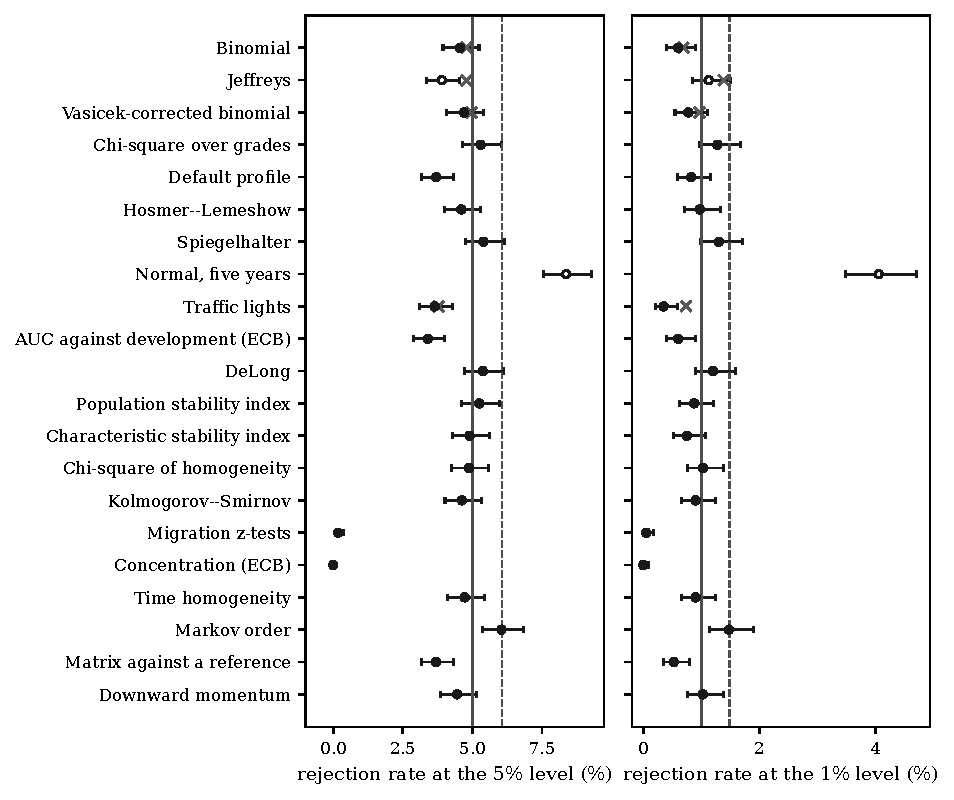
\includegraphics[width=\linewidth]{size_forest}
\caption{Measured size of the 21 credit-family tests at the 5\% level (left) and the 1\% level (right): the rate of the committed cell of 4,000 repetitions (circle) and the pooled rate of 200,000 repetitions (grey square), each with its Wilson 95\% interval, the level (solid line), the bound of the screen at 4,000 repetitions (dashed line), the exact rejection probability where it exists (cross), and open markers for the tests that do not hold their size on that evidence by \cref{def:holds}.}
\label{fig:size-forest}
\end{figure}

The other tests spread around their level and below it.
At 5\,\%, \nConsFive{} tests are conservative, with the whole Wilson interval below the level: the Jeffreys test at 5\,\% (exact \jeffExactFive\,\%), the default-profile test (\profileFive\,\%), the traffic-lights test (exact \tlLowerExact\,\%), the AUC test against the development AUC (\aucNullFive\,\%), the matrix test against a reference (\matFive\,\%), the migration z-tests (\migFive\,\%) and the concentration test (\hhiFive\,\%).
Two of these are conservative for a reason that is a property of the test and not of the sample: the migration z-tests control 42 cells at once with Holm's procedure, and the concentration statistic is bounded (\cref{prop:hhi}).
The binomial test is conservative because its count is discrete: its exact size at 5\,\% is \binExactFive\,\% and the simulated rate \binSimFive\,\% agrees with it.
The Markov-order test shows how the two rules part on one cell.
Its rate is \ordFive\,\% at 5\,\% against the bound of \boundFive\,\%, a margin of \markovBoundMargin\ points, so the screen passes it; but its Wilson interval, \ordLoFive\,\% to \ordHiFive\,\%, lies wholly above 5\,\%, and at 1\,\% its rate of \ordOne\,\% has an interval of \ordLoOne\,\% to \ordHiOne\,\%, wholly above 1\,\%, so by the definition it does not hold its size.
A run of 20,000 repetitions gives \ordTwentyK\,\% at 5\,\% with interval \ordTwentyKLo\,\% to \ordTwentyKHi\,\%, and the pool of the replication of \cref{sec:rs-seeds} \pooledOrd\,\%.
\Cref{fig:p-histograms} shows the p-values behind the rates: the binomial test has gaps where no count falls, the normal test piles its mass at small p-values, and the concentration test has all its mass at one, which is what a test that cannot reject looks like.

\begin{figure}[htbp]
\centering
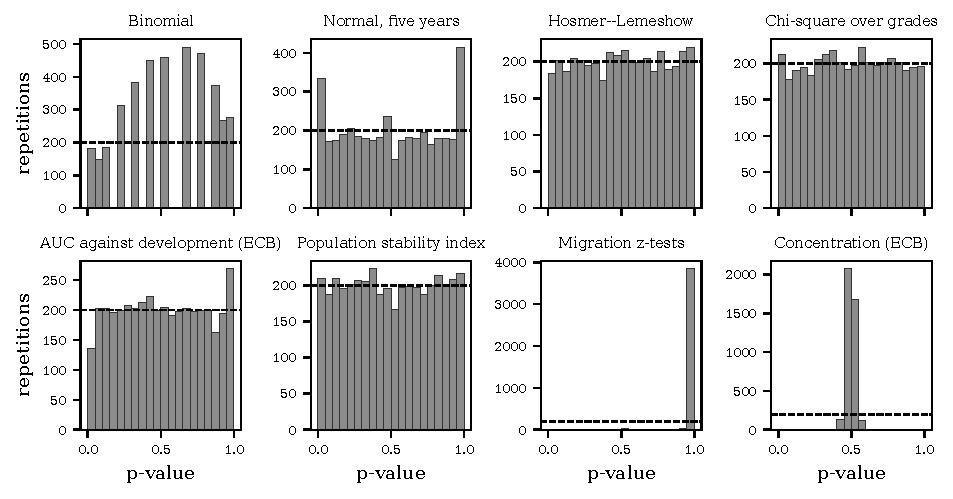
\includegraphics[width=\linewidth]{p_histograms}
\caption{Histograms of the p-values of eight tests under their null in 4,000 repetitions: a test that holds its size continuously has a flat histogram (dashed line), the discrete binomial test has empty bins, the normal test over five years has excess mass at small p-values, and the concentration test has all of its mass at one.}
\label{fig:p-histograms}
\end{figure}

\subsection{Settings that change a size}
\label{sec:rs-settings}

\Cref{tab:settings} lists the cells in which a setting of a test, and not a defect of the model, moves its size on the same generator.
Referring the Hosmer--Lemeshow statistic to two fewer degrees of freedom, as the original statistic does for a model fitted on the same sample, gives a size of \hlFitted\,\% at 5\,\% and \hlFittedOne\,\% at 1\,\% on a validation sample whose probabilities were not fitted on it, close to the \hlDofTheory\,\% of \cref{prop:reference}; with the degrees of freedom of the groups, the test has \hlFive\,\% and \hlOne\,\%.
The traffic-lights test measures \tlLowerExact\,\% exactly with the tie rule as printed and \tlUpperExact\,\% with the upper tie rule that the simulation of the Basel Committee must have used, so the rule that colours a year with exactly the expected number of defaults changes the size by two and a half points.
The chi-square test over grades rejects \chiThin\,\% at 5\,\% and \chiThinOne\,\% at 1\,\% when its best grade expects 0.6 defaults, above the bound at 1\,\%.
The AUC test against the development AUC rejects \aucDevOne\,\% at 5\,\% when the development AUC was estimated on a sample as large as the current one, against \aucDevOneExt\,\% when the variance of the development estimate is added, and \aucDevTheory\,\% is the prediction of \cref{prop:reference}.
The rules of thumb of the stability index, applied to two samples of 100 in which nothing changed, raise an alarm in \psiHundred\,\% of samples at 0.10 and \psiHundredTwentyFive\,\% at 0.25, against \psiHundredBench\,\% for its chi-square benchmark.

\begin{table*}[htbp]
\centering
\footnotesize
\caption{The settings of a test that change its measured size on the same null generator: Hosmer--Lemeshow with two fewer degrees of freedom, the traffic lights with the upper tie rule, a chi-square over a thin grade, the AUC test with an estimated development AUC and its extension, a longer run of the order test, and the PSI rules of thumb in samples of 100.}
\label{tab:settings}
\fitwidth{\begin{tabular}{p{2.4cm}p{4.6cm}rllcp{2.6cm}}
\toprule
Test & Setting & Reps & Size at 5\% [Wilson] & Size at 1\% & Exact 5\% / 1\% & Other rule \\
\midrule
Hosmer--Lemeshow & the same, with G $-$ 2 degrees of freedom (the model fitted on the same sample) & 4,000 & 10.97 [10.0, 12.0] & 3.38 & -- &  \\
Traffic lights & the upper tie rule WP14's simulation used & 4,000 & 6.35 [5.6, 7.1] & 1.40 & 6.03 / 1.13 &  \\
Chi-square over grades & a best grade expecting 0.6 defaults & 4,000 & 5.67 [5.0, 6.4] & 1.73 & -- &  \\
AUC against development (ECB) & the development AUC estimated on an equal sample (ECB form) & 4,000 & 11.58 [10.6, 12.6] & 4.52 & -- &  \\
AUC against development (ECB) & the same with the development AUC's variance added & 4,000 & 5.30 [4.6, 6.0] & 1.05 & -- &  \\
Markov order & the same chain, 20,000 repetitions: the order test's size measured to 0.15 points & 20,000 & 5.05 [4.8, 5.4] & 1.05 & -- &  \\
Population stability index & two samples of 100: the 0.10 and 0.25 rules of thumb & 4,000 & 6.98 [6.2, 7.8] & 2.05 & -- & PSI above 0.10: 85.0; above 0.25: 22.9 \\
\bottomrule
\end{tabular}}
\end{table*}


\subsection{Miscalibration and default clustering}
\label{sec:rs-defects}

\Cref{fig:power-calibration} shows the power of the nine calibration tests as the true probability of default rises above the one applied.
Each panel uses its own design, so the curves compare tests on the same panel and are not a ranking across panels.
On a portfolio of 5,000 obligors at 2\,\%, the binomial test rejects \binKOneTwoFive\,\% of samples when the true PD is 1.25 times the one applied (exact value \binKOneTwoFiveExact\,\%) and \binKOneFive\,\% at 1.5 times, and the Jeffreys test \jeffKOneTwoFive\,\% at 1.25.
On the obligor-level panel the Spiegelhalter test is the most powerful, with \spiKOneOne\,\% at 1.1 and \spiKOneTwoFive\,\% at 1.25 against \hlKOneOne\,\% and \hlKOneTwoFive\,\% for Hosmer--Lemeshow; on the panel of seven grades the chi-square test has \chiKOneOne\,\% and \chiKOneTwoFive\,\%.
Over five years the normal test rejects \normKOneTwoFive\,\% and the traffic-lights test \tlKOneTwoFive\,\% at 1.25.
Two curves show what correcting for a correlation costs and what a shape test cannot see.
The Vasicek-corrected binomial test, which assumes an asset correlation of 12\,\% that the generator does not have, rejects nothing at 1.25 or at 1.5 times and \vasKThree\,\% at three times (exact \vasKThreeExact\,\%).
The default-profile test rejects \profKThree\,\% when every probability of default is three times too low, its size, because it tests the shape of the curve and a uniform multiple leaves the shape unchanged.
The severity at which the curves of the tests that reach 80\,\% power cross it lies between \sSpi{} and \sHl{} times the PD applied for the seven tests of \cref{tab:power-summary} on these panels.

\begin{figure}[htbp]
\centering
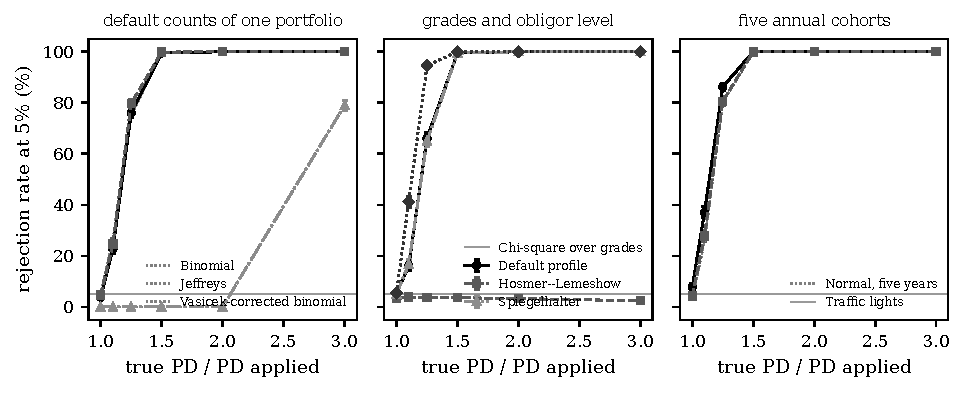
\includegraphics[width=\linewidth]{power_calibration}
\caption{Power at the 5\% level of the nine calibration tests against the ratio of the true probability of default to the one applied, in 2,000 repetitions per point with Wilson 95\% intervals; dotted lines are the exact rejection probabilities of the count tests and the traffic-lights test, which the simulated points follow.}
\label{fig:power-calibration}
\end{figure}

When the defaults are correlated and the probabilities of default are right, every rejection is a false alarm, and \cref{fig:clustering-size} shows how many.
At an asset correlation of 2\,\% the binomial test rejects \binRhoTwo\,\% of samples (exact \binRhoTwoExact\,\%), at 5\,\% it rejects \binRhoFive\,\% (exact \binRhoFiveExact\,\%), and at 10\,\% \binRhoOneZero\,\% (exact \binRhoOneZeroExact\,\%), against a level of 5\,\%, while the Vasicek-corrected test, whose assumed correlation is 12\,\%, holds its size near that correlation (\vasRhoOneZero\,\% at 10\,\%) and over-rejects beyond it (\vasRhoTwoZero\,\%, exact \vasRhoTwoZeroExact\,\%, at 20\,\%).
The tests built on grades and obligors fare worse: the chi-square test over grades rejects \chiRhoTwo\,\% at an asset correlation of 2\,\% and \chiRhoOneZero\,\% at 10\,\%, and Hosmer--Lemeshow \hlRhoTwo\,\% at 2\,\% and \hlRhoTwoZero\,\% at 20\,\%.
The normal test over five years goes the other way, from \normRhoZero\,\% at independence to \normRhoTwoZero\,\% at 20\,\%, because the year-to-year dispersion that it estimates absorbs the clustering.
A reader who sees a red light from a test that assumes independent defaults cannot tell a miscalibrated model from a correlated portfolio.

\begin{figure}[htbp]
\centering
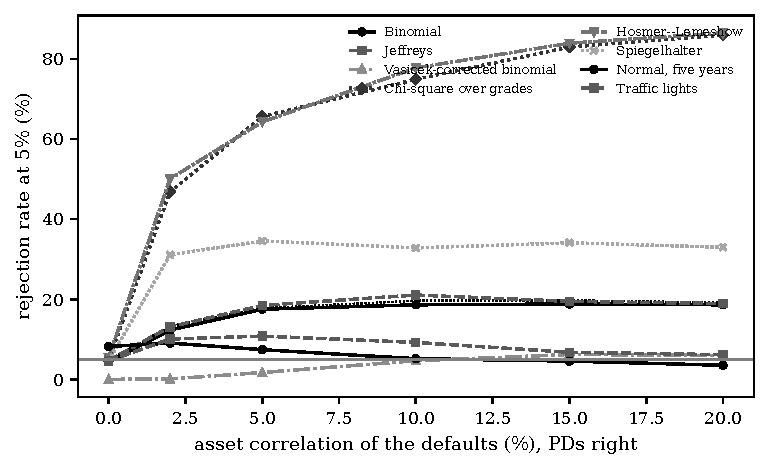
\includegraphics[width=0.85\linewidth]{clustering_size}
\caption{Rejection rate at 5\% of eight calibration tests when the probabilities of default are right and the defaults are correlated with the asset correlation on the horizontal axis, in 2,000 repetitions per point; the dotted line is the exact size of the binomial test, and every rejection above the level of 5\% is a false alarm.}
\label{fig:clustering-size}
\end{figure}

\subsection{Drift, discrimination, leakage and the rating system}
\label{sec:rs-stability}

\Cref{tab:power-summary} gives the power of the 17 tests along their ladders and \cref{fig:power-families} draws the curves of the other six defects.
For population drift of two samples of 1,000, the chi-square benchmark of the stability index has a power of \psiBenchZeroOne\,\% for a shift of 0.1 standard deviations and \psiBenchZeroTwo\,\% for 0.2; the chi-square test of homogeneity has \chiDriftZeroTwo\,\% at 0.2 and the Kolmogorov--Smirnov test \ksDriftZeroOne\,\% and \ksDriftZeroTwo\,\% at 0.1 and 0.2.
The fixed rules of thumb do not follow: at a shift of 0.2 the 0.10 rule alarms in \psiBandZeroOneAtZeroTwo\,\% and the 0.25 rule in \psiBandZeroTwoFiveAtZeroTwo\,\% of samples, and the 0.10 rule needs a shift of 0.3 to alarm in \psiBandZeroOneAtZeroThree\,\%.
The false alarm side of the same rules is in \cref{fig:psi-bands}: the measured rates of the printed study at the sample sizes in which nothing changed follow the asymptotic curve of \cref{prop:psi}.
A right model under a covariate shift stays calibrated, and the Hosmer--Lemeshow and Spiegelhalter tests reject \hlDriftZeroFive\,\% and \spiDriftZeroFive\,\% at a shift of 0.5 standard deviations, their size: drift and miscalibration are different questions.

\begin{figure}[htbp]
\centering
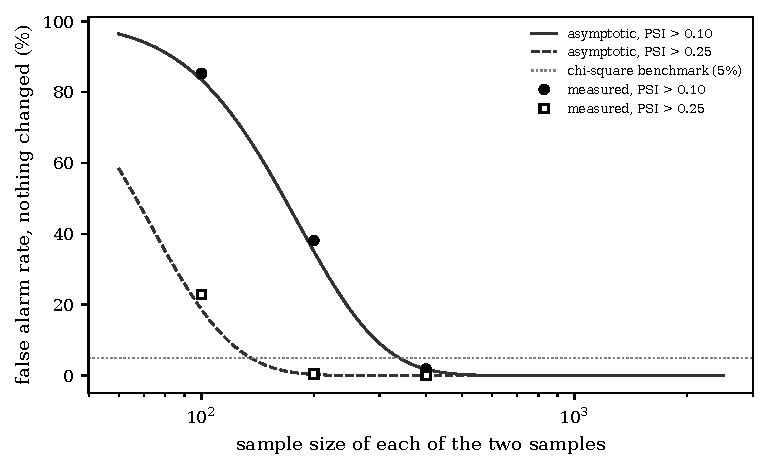
\includegraphics[width=0.85\linewidth]{psi_bands}
\caption{False alarm rate of the fixed bands of the population stability index when nothing changed, against the size of each of two samples: the asymptotic curves of the chi-square result for the bands 0.10 and 0.25, the 5\% of the chi-square benchmark, and the rates measured on the cells of the published study that the measurement reruns.}
\label{fig:psi-bands}
\end{figure}

For discrimination, with 150 defaulters, the ECB test against the development AUC rejects \ecbDropZeroTwo\,\% of samples for an AUC drop of two points, \ecbDropZeroFive\,\% for five and \ecbDropZeroEight\,\% for eight; DeLong's test, applied to a challenger whose AUC is lower by the same amount, rejects \delDropZeroTwo\,\% at two points and \delDropZeroFive\,\% at five, and it needs a drop of \delDropAtPower\ for 80\,\% power against \ecbDropAtPower\ for the ECB test.
Leakage of the outcome into a development feature is visible to the AUC test as a drop out of time, \leakAucZeroTwoFive\,\% at a shift of 0.25 and \leakAucZeroFive\,\% at 0.5, and almost invisible to the characteristic stability index of the leaked feature itself, which rejects \leakCsiZeroTwoFive\,\% at 0.25, \leakCsiOne\,\% at 1 and \leakCsiTwo\,\% at 2.
For the rating system, with 500 obligors per grade the migration z-tests reject \migROneFivenFiveZeroZero\,\% of samples when one cell is 1.5 times its closer neighbour, \migRTwonFiveZeroZero\,\% at twice and \migRThreenFiveZeroZero\,\% at three times; with 2,000 obligors the figures are \migROneFivenTwoZeroZeroZero\,\% at 1.5 and \migRTwonTwoZeroZeroZero\,\% at twice.
Swapping the default probabilities of two adjacent grades is seen by the default-profile test in \swapProfile\,\% of samples and by the chi-square test over grades in \swapChi\,\%.
The concentration test of the European Central Bank rejects \hhiPower\,\% of samples at every severity, including half of every grade's mass moved into the modal grade, where the chi-square test of homogeneity applied to the counts rejects \chiCountZeroZeroTwo\,\% at 2\,\% moved and \chiCountZeroZeroFive\,\% at 5\,\%.
\Cref{fig:hhi-bound} shows why: its statistic, computed exactly, stays below its critical value at every coefficient of variation.

\begin{table*}[htbp]
\centering
\footnotesize
\caption{Measured power at 5\%, in percent, of the 17 tests with a power curve at the six settings S1 to S6 of the ladder of the defect planted for each (2,000 repetitions per setting), and the setting at which the interpolated curve first reaches 80\% with the interval given by the Wilson limits of the points.}
\label{tab:power-summary}
\fitwidth{\begin{tabular}{llrrrrrrl}
\toprule
Test & Defect and ladder & S1 & S2 & S3 & S4 & S5 & S6 & Setting at 80\% power [95\%] \\
\midrule
Binomial & true PD / PD applied (1 to 3) & 3.8 & 22.8 & 76.0 & 99.6 & 100.0 & 100.0 & 1.29 [1.27, 1.31] \\
Jeffreys & true PD / PD applied (1 to 3) & 4.7 & 24.7 & 79.8 & 99.9 & 100.0 & 100.0 & 1.25 [1.25, 1.27] \\
Vasicek-corrected binomial & true PD / PD applied (1 to 3) & 0.0 & 0.0 & 0.0 & 0.0 & 0.0 & 79.0 & not reached \\
Chi-square over grades & true PD / PD applied (1 to 3) & 5.3 & 16.0 & 66.1 & 99.5 & 100.0 & 100.0 & 1.35 [1.34, 1.36] \\
Default profile & true PD / PD applied (1 to 3) & 3.3 & 3.9 & 3.8 & 3.6 & 3.2 & 2.4 & not reached \\
Hosmer--Lemeshow & true PD / PD applied (1 to 3) & 5.0 & 16.8 & 64.9 & 99.5 & 100.0 & 100.0 & 1.36 [1.35, 1.37] \\
Spiegelhalter & true PD / PD applied (1 to 3) & 5.3 & 41.2 & 94.6 & 100.0 & 100.0 & 100.0 & 1.21 [1.21, 1.21] \\
Normal, five years & true PD / PD applied (1 to 3) & 7.8 & 37.0 & 86.2 & 100.0 & 100.0 & 100.0 & 1.23 [1.23, 1.24] \\
Traffic lights & true PD / PD applied (1 to 3) & 4.3 & 27.8 & 80.6 & 100.0 & 100.0 & 100.0 & 1.25 [1.24, 1.26] \\
AUC against development (ECB) & AUC drop (0 to 0.08) & 2.9 & 11.6 & 25.4 & 46.2 & 81.5 & 99.1 & 0.0492 [0.0482, 0.0505] \\
DeLong & AUC drop (0 to 0.08) & 4.9 & 8.1 & 18.0 & 34.2 & 71.6 & 97.8 & 0.0596 [0.0578, 0.0614] \\
Population stability index & mean shift (standard deviations) (0 to 0.5) & 5.0 & 9.6 & 27.2 & 89.6 & 100.0 & 100.0 & 0.185 [0.182, 0.187] \\
Characteristic stability index & leak (shift of the feature for defaulters) (0 to 2) & 4.7 & 6.0 & 7.8 & 14.6 & 33.4 & 58.1 & not reached \\
Chi-square of homogeneity & mean shift (standard deviations) (0 to 0.5) & 4.6 & 9.3 & 26.2 & 88.5 & 100.0 & 100.0 & 0.186 [0.184, 0.189] \\
Kolmogorov--Smirnov & mean shift (standard deviations) (0 to 0.5) & 5.5 & 14.9 & 46.5 & 97.3 & 100.0 & 100.0 & 0.166 [0.164, 0.168] \\
Migration z-tests & planted cell / closer neighbour (1 to 4) & 0.1 & 1.3 & 7.9 & 55.5 & 99.7 & 100.0 & 2.55 [2.53, 2.58] \\
Concentration (ECB) & share moved into the modal grade (0 to 0.5) & 0.0 & 0.0 & 0.0 & 0.0 & 0.0 & 0.0 & not reached \\
\bottomrule
\end{tabular}}
\end{table*}


\begin{figure}[htbp]
\centering
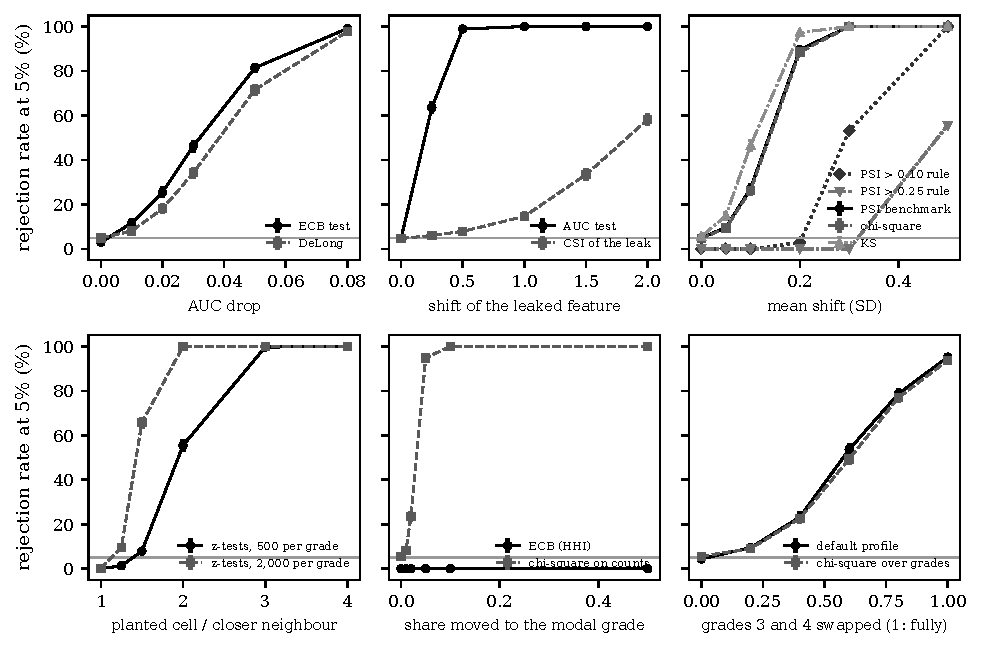
\includegraphics[width=\linewidth]{power_families}
\caption{Power at 5\% against the planted defect of the tests of discrimination decay, leakage, drift, broken monotonicity of the migrations, concentration and swapped grades, with Wilson 95\% intervals in 2,000 repetitions per point; drift also shows the rules of thumb PSI above 0.10 and above 0.25, which never reach the power of the benchmark.}
\label{fig:power-families}
\end{figure}

\begin{figure}[htbp]
\centering
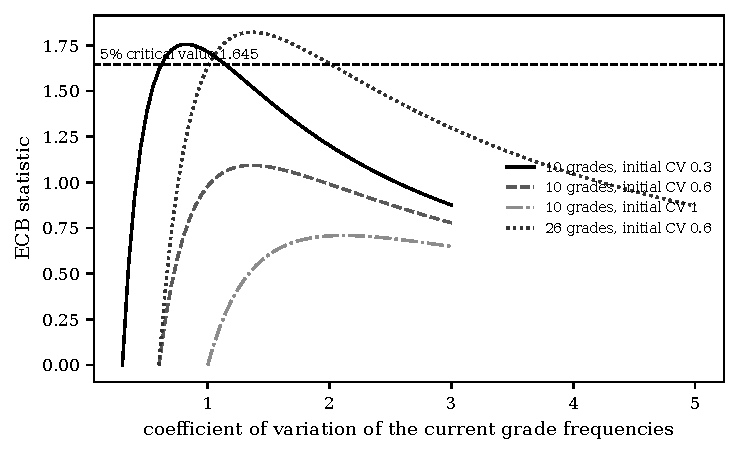
\includegraphics[width=0.85\linewidth]{hhi_bound}
\caption{The concentration statistic of the European Central Bank as a function of the current coefficient of variation of the grade frequencies, computed exactly for 10 grades with initial coefficients of variation 0.3, 0.6 and 1 and for 26 grades with 0.6; only the curves that rise above the dashed critical value of 1.645 can reject at 5\%.}
\label{fig:hhi-bound}
\end{figure}

Of the \nPowerTests{} curves, \nReach{} reach 80\,\% on their ladder.
The four that do not are the Vasicek-corrected binomial test (\vasKThree\,\% at the top of its ladder, within the Monte Carlo error of 80\,\%), the default-profile test against a uniform multiple of the probabilities, the characteristic stability index against a leak, and the concentration test.
For the ones that do, the severity at which the curve crosses 80\,\% is in \cref{tab:power-summary}: for example an AUC drop of \ecbDropAtPower, a mean shift of \sPsi, \sChiStab{} and \sKs{} standard deviations for the benchmark of the stability index, the chi-square test of homogeneity and the Kolmogorov--Smirnov test, and a planted migration cell \sMig{} times its closer neighbour for 500 obligors per grade.

\subsection{The instrument: exact values, published studies and reproduction}
\label{sec:rs-instrument}

The exact rejection probabilities of \nExactRows{} rows give \nExactCmp{} comparisons with the simulated rates at two levels, and all \nAgree{} agree within 3.29 standard errors by \eqref{eq:agree}; the largest absolute $z$ is \zMaxAbs.
Over the \nExactNondeg{} comparisons whose exact probability lies between 0.5\,\% and 99.5\,\%, where a rate can differ from it, the mean of $z$ is \zMean{} and its standard deviation \zSd, above one; the two levels of a row share their draws, so the values are not independent and their standard deviation is less precise than for independent values, and none exceeds 3.29.
A routine that calls no function of the engine and recomputes the exact rejection probability of the binomial test from the configuration of each generator reproduces \nBinRecon{} of the committed exact values to $\binReconMax$.
No power curve falls by more than 3.29 combined standard errors between neighbouring severities: \nMonoViol{} violations in \nMonoPairs{} adjacent pairs, against the expected 0.1 of \cref{sec:th-monotone}.

The reruns of the published studies are in \cref{tab:reproductions} and \cref{fig:reproductions}.
The rerun agrees with \wpAgree{} of the \wpTotal{} cells of the normal and traffic-lights tests of the Basel Committee at \wpRuns{} runs; the one cell that does not, the traffic-lights test in the scenario labelled DV\_LV at the 0.1\,\% level, is printed as \wpOffPub\,\% and measured as \wpOffMeas\,\%.
It agrees with \ynAgree{} of the \ynTotal{} cells of the stability study at \ynRuns{} runs; the harness sits slightly above the printed rates, with a mean $z$ of $+\ynMeanZ$ over the \ynInterior{} cells whose printed rate is strictly between 0 and 1.
The nested-model rate of the DeLong test is \demlerMeasured\,\% in \demlerRuns{} runs against the printed \demlerPublished\,\%.
Every one of the \nReproTotal{} committed null cells reproduces exactly: the counts of rejections, at both levels, and the number of undefined results equal the committed ones when the cell is rerun from its configuration and its seed.
The estimators that the harness also measures agree: the AUC of 4,000 binormal samples has a normal interval that covers \aucCover\,\% of the time (Monte Carlo standard error \aucCoverMcse\,\%), and the standard error of the ECB formula differs from the empirical one by $\aucSeRel\,\%$.

\begin{table*}[htbp]
\centering
\footnotesize
\caption{The three published simulation studies rerun by the measurement: the runs of the study and of the rerun, the cells whose printed rate agrees with the measured one within 3.29 pooled standard errors, the mean z of the differences, and each cell that disagrees.}
\label{tab:reproductions}
\fitwidth{\begin{tabular}{p{4.2cm}rrrp{5.3cm}}
\toprule
Published study & Runs: printed / ours & Cells agreeing & Mean z & Cells that disagree \\
\midrule
BCBS WP14 Tables 7 and 8: the normal and traffic-lights tests & 25,000 / 25,000 & 143 of 144 & -0.11 & DV\_LV, traffic, 0.001: printed 0.955, measured 0.9436 \\
Yurdakul and Naranjo (2020) Table 4: the PSI's rules and benchmark & 10,000 / 10,000 & 50 of 54 & +0.67 & m 100, n 400, shift 0.25 SD, PSI $>$ 0.10: printed 0.834, measured 0.8522; m 100, n 400, shift 0.5 SD, PSI $>$ 0.25: printed 0.787, measured 0.8098; m 200, n 200, shift 0 SD, chi-square: printed 0.057, measured 0.0688; m 200, n 400, shift 0.5 SD, PSI $>$ 0.25: printed 0.72, measured 0.7421 \\
Demler, Pencina and D'Agostino (2012): DeLong on nested models & 1,000 / 1,000 & 1 of 1 & +0.58 & none \\
\bottomrule
\end{tabular}}
\end{table*}


\begin{figure}[htbp]
\centering
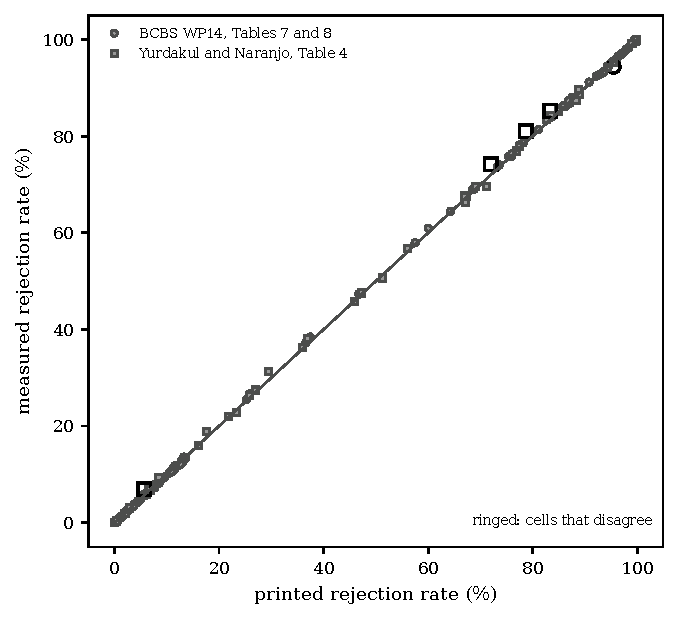
\includegraphics[width=0.7\linewidth]{reproductions}
\caption{Printed rejection rate against the rate measured by the rerun, for the 144 cells of the Basel Committee's study of the normal and traffic-lights tests and the 54 cells of the stability index study; the diagonal is agreement and the ringed points are the cells that do not agree within 3.29 pooled standard errors.}
\label{fig:reproductions}
\end{figure}

\subsection{Replication across seeds}
\label{sec:rs-seeds}

\Cref{tab:seed-replication} and \cref{fig:seed-spread} report the \nBlocks{} independent blocks of each test.
The Monte Carlo standard error is calibrated: the standard deviation of the block rates over the binomial standard error, $\kappa$ of \eqref{eq:kappa}, has a mean of \sdRatioMean{} over tests and levels, with a range from \sdRatioMin{} to \sdRatioMax{}, as fifty blocks allow.
The pooled sizes sort the tests into three groups: \nWithin{} lie within the level (the pooled rate does not exceed it at either level), \nOver{} lie above it (the lower Wilson limit of the pooled rate exceeds the level at one level), and \nNeither{} are in neither, with a pooled rate slightly above the level at one level and an interval that includes it (the chi-square test of homogeneity and the downward-momentum test).
The tests of the third group hold their size by \cref{def:holds}, so that the tests of the first and third groups, \nHold{} in all, hold their size on the pool and the \nOver{} of the second do not.
Among the \nOver{} are the two tests that the committed cells flag by the screen, and \nSmallOver{} others whose excess, at the level that places them above, is small: the stability index at \pooledPsi\,\% at 5\,\%, Hosmer--Lemeshow at \pooledHl\,\% (and \pooledHlOne\,\% at 1\,\%), the Spiegelhalter test, the Markov-order test and the chi-square test over grades (respectively \pooledSpi\,\%, \pooledOrd\,\% and \pooledChi\,\% at 5\,\%), DeLong at \pooledDel\,\% at 5\,\% and the characteristic stability index at \pooledCsiOne\,\% at 1\,\% (its 5\,\% rate, \pooledCsi\,\%, has an interval that includes the level); the excesses range from \smallExcMin{} to \smallExcMax{} points, below what a cell of \nNullReps{} repetitions can resolve (\detIntFiveFour{} points at 5\,\%).
The judgement of the committed cell equals that of the pool, both by \cref{def:holds}, for \nVerdictAgree{} of the \nTests{} tests and differs for \nVerdictDisagree{}, the tests that the pool shows above their level and the cell does not; by the screen the figures are \nVerdictAgreeRule{} and \nVerdictDisagreeRule{}.
The normal test pools to \pooledNorm\,\% and the Jeffreys test to \pooledJeffOne\,\% at 1\,\%, the exact value.

\begin{table*}[htbp]
\centering
\footnotesize
\caption{Fifty independent blocks of 4,000 repetitions (200,000 in all) for each of the 21 tests: the committed cell, the pooled rate with its Wilson interval, the standard deviation of the block rates beside the binomial standard error at 5\%, the share of blocks flagged by the one-sided bound and by the rule that a rate above the level is oversized, and the judgement of the committed cell and of the pool.}
\label{tab:seed-replication}
\fitwidth{\begin{tabular}{lrlcrrlcc}
\toprule
Test & Cell 5\% & Pooled 5\% [Wilson] & SD / SE of blocks & Flagged: bound / naive (\%) & Cell 1\% & Pooled 1\% [Wilson] & Cell holds & Pooled holds \\
\midrule
Binomial & 4.55 & 4.81 [4.72, 4.91] & 0.33 / 0.34 & 0 / 26 & 0.60 & 0.66 [0.62, 0.69] & yes & yes \\
Jeffreys & 3.90 & 4.71 [4.62, 4.81] & 0.32 / 0.34 & 0 / 18 & 1.12 & 1.38 [1.33, 1.43] & no & no \\
Vasicek-corrected binomial & 4.70 & 4.92 [4.82, 5.01] & 0.42 / 0.34 & 0 / 44 & 0.78 & 1.00 [0.95, 1.04] & yes & yes \\
Chi-square over grades & 5.30 & 5.15 [5.06, 5.25] & 0.37 / 0.35 & 2 / 64 & 1.27 & 1.21 [1.16, 1.26] & yes & no \\
Default profile & 3.70 & 4.05 [3.97, 4.14] & 0.29 / 0.31 & 0 / 0 & 0.83 & 0.76 [0.72, 0.80] & yes & yes \\
Hosmer--Lemeshow & 4.60 & 5.17 [5.08, 5.27] & 0.31 / 0.35 & 0 / 68 & 0.97 & 1.26 [1.21, 1.31] & yes & no \\
Spiegelhalter & 5.40 & 5.15 [5.06, 5.25] & 0.32 / 0.35 & 0 / 66 & 1.30 & 1.10 [1.06, 1.15] & yes & no \\
Normal, five years & 8.38 & 7.99 [7.87, 8.11] & 0.40 / 0.43 & 100 / 100 & 4.05 & 3.56 [3.48, 3.64] & no & no \\
Traffic lights & 3.65 & 3.81 [3.73, 3.90] & 0.30 / 0.30 & 0 / 0 & 0.35 & 0.73 [0.70, 0.77] & yes & yes \\
AUC against development (ECB) & 3.40 & 4.00 [3.91, 4.08] & 0.28 / 0.31 & 0 / 0 & 0.60 & 0.63 [0.59, 0.66] & yes & yes \\
DeLong & 5.38 & 5.13 [5.03, 5.23] & 0.31 / 0.35 & 0 / 68 & 1.20 & 1.03 [0.99, 1.08] & yes & yes \\
Population stability index & 5.25 & 5.29 [5.19, 5.38] & 0.43 / 0.35 & 4 / 78 & 0.88 & 1.10 [1.06, 1.15] & yes & no \\
Characteristic stability index & 4.90 & 5.09 [5.00, 5.19] & 0.35 / 0.35 & 2 / 60 & 0.75 & 1.05 [1.00, 1.09] & yes & yes \\
Chi-square of homogeneity & 4.88 & 5.00 [4.91, 5.10] & 0.39 / 0.34 & 0 / 48 & 1.03 & 1.00 [0.96, 1.04] & yes & yes \\
Kolmogorov--Smirnov & 4.62 & 4.87 [4.78, 4.96] & 0.30 / 0.34 & 0 / 30 & 0.90 & 0.99 [0.95, 1.03] & yes & yes \\
Migration z-tests & 0.18 & 0.11 [0.10, 0.13] & 0.05 / 0.05 & 0 / 0 & 0.05 & 0.02 [0.02, 0.03] & yes & yes \\
Concentration (ECB) & 0.00 & 0.00 [0.00, 0.00] & 0.00 / 0.00 & 0 / 0 & 0.00 & 0.00 [0.00, 0.00] & yes & yes \\
Time homogeneity & 4.72 & 4.35 [4.26, 4.44] & 0.31 / 0.32 & 0 / 0 & 0.90 & 0.78 [0.74, 0.81] & yes & yes \\
Markov order & 6.05 & 5.15 [5.05, 5.25] & 0.35 / 0.35 & 0 / 62 & 1.47 & 1.11 [1.07, 1.16] & yes & no \\
Matrix against a reference & 3.70 & 3.34 [3.27, 3.42] & 0.30 / 0.28 & 0 / 0 & 0.53 & 0.62 [0.58, 0.65] & yes & yes \\
Downward momentum & 4.45 & 4.98 [4.89, 5.08] & 0.35 / 0.34 & 0 / 46 & 1.03 & 1.01 [0.97, 1.06] & yes & yes \\
\bottomrule
\end{tabular}}
\end{table*}


\begin{figure}[htbp]
\centering
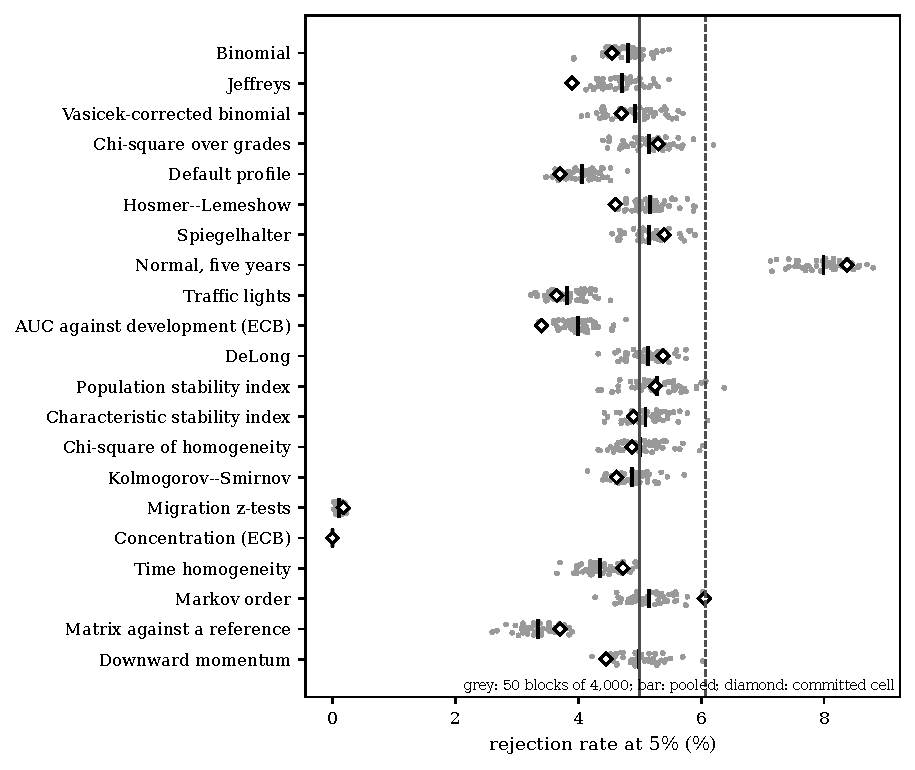
\includegraphics[width=\linewidth]{seed_spread}
\caption{Rejection rate at 5\% of each of the 21 tests in 50 independent blocks of 4,000 repetitions (grey points), the pooled rate (vertical bar) and the committed cell (diamond); the solid line is the level and the dashed line the bound of a cell of 4,000 repetitions.}
\label{fig:seed-spread}
\end{figure}

\subsection{The 21 tests outside the credit families}
\label{sec:extension}

The engine registers \nExtTests{} further p-value tests of counterparty credit risk, provisioning, loss given default, market risk, portfolio credit risk, fairness and machine learning, which it measures through \nStudies{} named studies, each with a generator of the null and one stated alternative.
\Cref{tab:extension} and \cref{fig:extension} give the size of each at 4,000 repetitions and its power against its one alternative at 2,000.
By \cref{def:holds} on cells of \nNullReps{} repetitions, \nExtHold{} of the \nExtTests{} tests hold their size at both levels, and \nStudiesHold{} of the \nStudies{} studies; the screen passes \nExtHoldRule{} tests and \nStudiesHoldRule{} studies.
The \nStudiesNotHold{} studies that do not hold are the independence test and the conditional-coverage test of Christoffersen, at the series length of 1,500 days at 5\,\% (the independence test rejects \chrIndFive\,\% at 5\,\% and \chrIndOne\,\% at 1\,\%, and the conditional-coverage test \chrCcFive\,\% at 5\,\%), the calibration of the loss given default over time (\lgdTimeOne\,\% at 1\,\%), the convergence of the Monte Carlo quantile, whose excess the engine documents (\mcConvFive\,\% at 5\,\%), and the unconditional test of Du and Escanciano (\duUncondFive\,\% at 5\,\%).
These are single cells without a replication, so each judgement carries the resolution of \detIntFiveFour{} points, and at most about \expFalseAboveExt{} of the 25 studies would be shown above their level by chance if every study had exactly its level.
Among these tests are the residual test of \citet{mcneil2000}, the duration test of \citet{christoffersen2004}, the expected-shortfall tests of \citet{acerbi2014} and \citet{du2017}, the dynamic quantile test of \citet{engle2004}, and the recursion for CreditRisk+ \citep{haaf2004} that the study compares with a Monte Carlo run.
At 5\,\%, \nExtCons{} studies are conservative, with the whole interval below the level.
Against its stated alternative the power at 5\,\% runs from \extPowMin\,\% to \extPowMax\,\% with a median of \extPowMed\,\%; \extAboveBar{} studies reach 80\,\% and \extBelowHalf{} detect their alternative less than half of the time.
These alternatives are the engine's choices, one departure for each test, and the powers are not comparable across tests.

\begin{table}[htbp]
\centering
\footnotesize
\caption{The 25 named studies of the 21 tests outside the credit families: the measured size at 5\% and 1\% (4,000 repetitions) on the null of each study, whether both sizes lie within the one-sided bound, and the power at 5\% against the one alternative the study states (2,000 repetitions), in percent.}
\label{tab:extension}
\fitwidth{\begin{tabular}{p{7.4cm}rrcr}
\toprule
Study & Size at 5\% & Size at 1\% & Holds & Power at 5\% $\pm$ SE \\
\midrule
PFE exceedance back-test, PFE at 95\%, 1,000 dates & 5.25 & 1.23 & yes & 72.5 $\pm$ 1.0 \\
IFRS 9 stage-migration back-test, three stages, 4,000, 1,500 and 500 accounts & 4.75 & 1.10 & yes & 74.9 $\pm$ 1.0 \\
LGD calibration by segment, one segment, 250 workouts & 4.67 & 0.78 & yes & 82.4 $\pm$ 0.9 \\
LGD calibration over time, five default years, 60 workouts each & 5.12 & 1.47 & yes & 57.6 $\pm$ 1.1 \\
Downturn LGD coverage, 150 downturn workouts, estimate 0.45 & 5.42 & 1.25 & yes & 67.1 $\pm$ 1.1 \\
McNeil--Frey residual test, 2,500 days at 5\%, 125 exceedances expected & 3.57 & 0.43 & yes & 93.2 $\pm$ 0.6 \\
Tail back-test (LHP quantile), 60 years at the 95\% level & 3.57 & 1.15 & yes & 30.1 $\pm$ 1.0 \\
Tail back-test (LHP quantile), 250 years at the 99\% level & 4.20 & 0.35 & yes & 96.0 $\pm$ 0.4 \\
Monte Carlo quantile convergence, 20,000 scenarios, the 99\% quantile of the LHP loss rate & 5.88 & 1.32 & yes & 74.6 $\pm$ 1.0 \\
CreditRisk+ recursion against Monte Carlo, 2,000 scenarios, 400 obligors in five exposure bands & 3.02 & 0.73 & yes & 55.8 $\pm$ 1.1 \\
Two-proportion z (fairness), 2,000 applicants, two groups & 5.47 & 0.92 & yes & 99.0 $\pm$ 0.2 \\
Fisher exact (fairness), 2,000 applicants, two groups & 4.52 & 1.05 & yes & 98.6 $\pm$ 0.3 \\
Kupiec proportion of failures, 1,500 days at 5\% & 4.80 & 0.83 & yes & 69.3 $\pm$ 1.0 \\
Christoffersen independence, 1,500 days at 5\% & 5.67 & 1.52 & \textbf{no} & 87.5 $\pm$ 0.7 \\
Christoffersen conditional coverage, 1,500 days at 5\% & 6.90 & 1.43 & \textbf{no} & 81.2 $\pm$ 0.9 \\
Duration test, 400 days at 5\% & 3.92 & 0.00 & yes & 59.7 $\pm$ 1.1 \\
Acerbi--Sz\'ekely ES test, 250 days at 2.5\% & 4.92 & 1.20 & yes & 89.4 $\pm$ 0.7 \\
Du--Escanciano, unconditional, 2,000 days at 10\% & 5.78 & 1.38 & yes & 56.5 $\pm$ 1.1 \\
Du--Escanciano, conditional, 2,000 days at 10\% & 4.85 & 1.10 & yes & 73.2 $\pm$ 1.0 \\
Dynamic quantile test, 1,500 days at 5\% & 4.00 & 0.00 & yes & 71.0 $\pm$ 1.0 \\
Dynamic quantile test, 250 days at 1\% & 4.42 & 0.00 & yes & 14.0 $\pm$ 0.8 \\
Dynamic quantile test, 250 days at 2.5\% & 4.23 & 0.00 & yes & 23.8 $\pm$ 1.0 \\
Dynamic quantile test, 750 days at 1\% & 3.43 & 0.00 & yes & 26.2 $\pm$ 1.0 \\
Shift resilience (ML), 2,000 development rows, a quarter worst-subsample share & 4.95 & 0.00 & yes & 97.0 $\pm$ 0.4 \\
Conformal coverage (ML), 2,000 test rows, 90\% coverage & 4.60 & 0.97 & yes & 100.0 $\pm$ 0.0 \\
\bottomrule
\end{tabular}}
\end{table}


\begin{figure}[htbp]
\centering
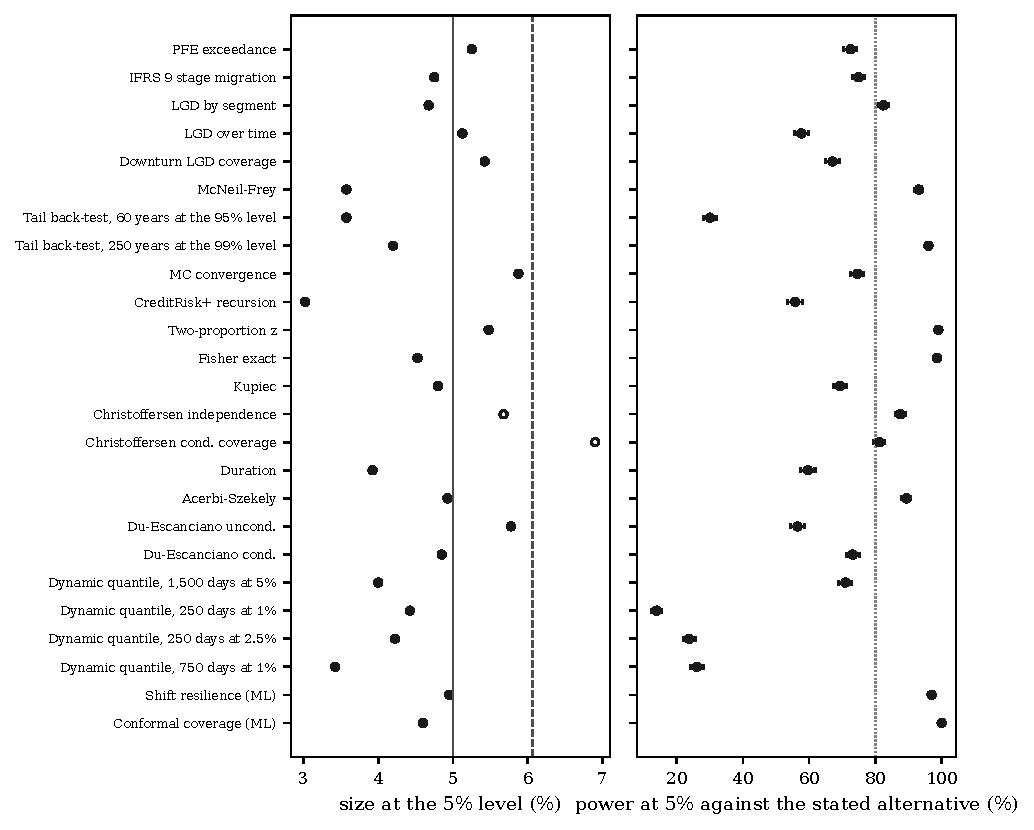
\includegraphics[width=\linewidth]{extension}
\caption{Size at 5\% (left, with the level as a solid line and the one-sided bound as a dashed line) and power at 5\% against the one alternative that each study states (right, with Wilson 95\% intervals and a dotted line at 80\%) for the 25 studies of the 21 tests outside the credit families.}
\label{fig:extension}
\end{figure}

\subsection{Whether each prediction held}
\label{sec:rs-hypotheses}

\Cref{tab:outcomes} reports the eight predictions of \cref{tab:predictions} against their criteria.
Five held and three are refuted.
P2 is refuted: \nNotHoldCellDef{} of the \nTests{} tests do not hold their size on the committed cells and \nNotHold{} do not on the pool.
P7 is refuted: the judgement of one cell of \nNullReps{} repetitions differs from that of the pool for \nVerdictDisagree{} tests.
P8 is refuted: \nNoReach{} of the \nPowerTests{} power curves do not reach 80\,\% on their ladder. The three refutations have three different causes. P2 fails because of \nNotHold{} tests on the pool: two with the largest excess and two different mechanisms, a Bayesian posterior used as a frequentist test of a discrete count and an aggregate over five years whose oversizing the simulation of the Basel Committee also shows, and \nSmallOver{} more with small excesses, of which the Markov-order test is already shown by the committed cell. P7 fails because the resolution of a cell is coarser than the excesses that \nVerdictDisagree{} tests have, of \smallExcMin{} to \smallExcMax{} points. P8 fails because four tests do not respond to the defect planted for them within the ladder, which is a statement about the pair of test and ladder.

\begin{table}[htbp]
\centering
\footnotesize
\caption{Outcome of each prediction of the measurement against its criterion, with the numbers from the committed documents and the experiments; P2, P7 and P8 are refuted, the other five hold.}
\label{tab:outcomes}
\fitwidth{\begin{tabular}{p{0.8cm}p{5.4cm}p{6.5cm}p{1.4cm}}
\toprule
ID & Criterion & Measured & Outcome \\
\midrule
P1 & 21 sizes, 17 curves, every rate with its error & \nSims{} simulations, \nRates{} rates, all with standard error and Wilson interval; 4 transition tests with a size only & held \\
P2 & 21 of 21 tests hold their size, by \cref{def:holds} & \nHoldCellDef{} of 21 hold on the cells of 4,000 repetitions (\nHoldCellRule{} pass the screen) and \nHold{} on the pool of 200,000; Jeffreys at 1\,\% (exact \jeffExactOne\,\%) and the normal test over five years (\normFive\,\%) do not hold on either & refuted \\
P3 & all exact comparisons agree & \nAgree{} of \nExactCmp{}, largest $|z|$ \zMaxAbs & held \\
P4 & at least 143 of 144, 48 of 54, and the nested-model rate & \wpAgree{} of \wpTotal{}, \ynAgree{} of \ynTotal{}, \demlerMeasured\,\% against \demlerPublished\,\% & held \\
P5 & no fall of more than 3.29 combined standard errors & \nMonoViol{} of \nMonoPairs{} pairs & held \\
P6 & every committed count reproduces & \nReproduced{} of \nReproTotal{} cells exact & held \\
P7 & one cell and the pool judge every test alike, by \cref{def:holds} & \nVerdictAgree{} of 21 agree (\nVerdictAgreeRule{} by the screen) & refuted \\
P8 & every power curve reaches 80\,\% & \nReach{} of \nPowerTests{} reach it & refuted \\
\bottomrule
\end{tabular}}
\end{table}
